\documentclass[a4paper]{article}
\usepackage[a4paper,pdftex]{geometry}
\usepackage[english]{babel}
\usepackage{amsmath,amsfonts}
\usepackage[pdftex]{graphicx}
\usepackage{epstopdf}
\usepackage{fancyhdr}
\usepackage{lastpage}
\usepackage{setspace}

% Page margins
%\setlength{\oddsidemargin}{5mm}
%\setlength{\evensidemargin}{5mm}

% Page style
\pagestyle{plain}

% Page numbering
\lhead{Sensor Fusion on a mini Unmanned Vehicles - Camiel R. Verschoor}
\cfoot{}
\rfoot{\thepage}

% TITLE FORMAT
\newcommand{\HRule}[1]{\rule{\linewidth}{#1}}

\makeatletter
\def\printtitle{
    {\centering \@title\par}}
\makeatother                  

\makeatletter
\def\printauthor{
    {\centering \large \@author}}
\makeatother

% TITLE
\title{
\HRule{0.5pt} \\
\LARGE \textbf{\textsc{Sensor Fusion on a mini Unmanned Vehicle}}\\[0.5cm]
\normalsize \textsc{Integrating vision-based algorithms on an AscTec Pelican to autonomously follow linear shaped structures in a landscape.}
\HRule{2pt}\\ [0.5cm]
Camiel R. Verschoor\\
10017321\\
\vspace{1cm}
Bachelor thesis\\
Credits: 18 EC\\
\vspace{0.5cm}
Bachelor Opleiding Kunstmatige Intelligentie\\
\vspace{0.25cm}
University of Amsterdam\\
Faculty of Science\\
Science Park 904\\
1098 XH Amsterdam\\
}

% AUTHOR
\author{\normalsize
\emph{Supervisors}\\
Dr. A. Visser\\
\vspace{0.25cm}
Informatics Institute\\
Faculty of Science\\
University of Amsterdam\\
Science Park 904\\
1098 XH  Amsterdam\\
\vspace{0.5cm}
Drs. G. Poppinga\\
\vspace{0.25cm}
Aerospace Systems (ASD)\\
Defense Systems (ASMO)\\
National Aerospace Lab\\
Anthony Fokkerweg 2\\
1059 CM Amsterdam\\
\vspace{1cm}
July 24th, 2012\\
}

% BEGIN DOCUMENT
\begin{document}

% TITLE PAGE
\thispagestyle{empty}
\printtitle
\vfill          
\printauthor
\newpage

% ABSTRACT
\section*{Abstract}
To be written.
\section*{Acknowledgements}
To be written.
\newpage

% TABLE OF CONTENTS
\tableofcontents
\newpage

\section{Introduction}
\onehalfspace
In robotics one of the main goals is to develop mobile robots that can operate autonomously in the real world environment. These autonomous robots have various purposes and are used for a wide range of applications such as inspection, exploration and rescue. In rescue, robots are expected to operate in dangerous environments without putting human lives at risk in example, during disasters or life rescue operations. Even though reasonable developments have been made in the robotics field, robots cannot operate autonomously in the real world yet.

One of the main requirements of an autonomous robot is the ability to navigation in the environment. The traditional approach to navigate through the outdoor environment is via pre-planned paths based on a Global Positioning System (GPS). The main shortcoming of GPS is that it cannot be used in every environment as it needs to receive data signals from four different satellites. Inside buildings and in several outdoor areas GPS is not available. In urban areas GPS is found to be especially unreliable. In order to navigate through these environments other sensors and navigation techniques need to be applied. Since there are several linear structures in the environment such as rivers, roads and power lines, line-following is one possible approach to navigate through an environment. Line-following is a classic technique in robotics as it has been successfully used for ground robots numerous times. For other robots and sensor configurations, open problems still remain. One of these is navigation for micro aerial vehicles (MAVs), which have a limited sensor composition due to their limited payload.

\begin{figure}[!h]
	\centering
	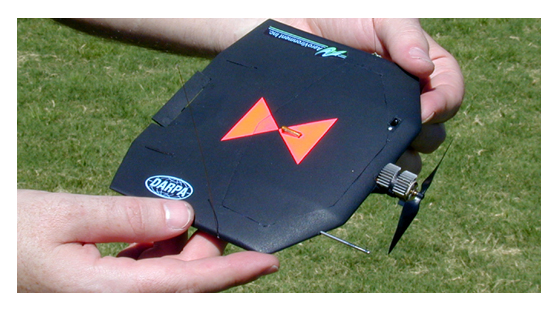
\includegraphics[width=0.5\textwidth]{images/blackwidow.eps}
	\caption{The Black Widow was the first operating micro aerial vehicle system developed by AeroVironment for Defense Advanced Research Projects Agency (DARPA). The Black Widow can fly for up to 20 minutes and carries a very small color video camera.}
	\label{blackwidow}
\end{figure}

A micro aerial vehicle (MAV) is a subclass of the Unmanned Aerial Vehicles. Due to their small size, the MAV can operate in numerous robotic applications, for instance, search \&  rescue, inspection and exploration. AeroVironment Black Widow (figure \ref{blackwidow}) is the first MAV operating in the field. Another type of MAV is the quadrotor, which is controlled by four rotors. Quadrotors provide manoeuvrability and stability, which is suitable for indoor and urban flights. As a result of recent developments, small quadrotors with on-board stabilization can be purchased conveniently. Due to this, the research regarding this platform is moving towards intelligent applications, which demand information of the surrounding environment. Nevertheless, the fast movements and the limited amount of sensor combination mean that it is still a challenge to develop navigation methods for these platforms.

\subsection{Platform and Framework}
The Ascending Technologies Pelican better known as the AscTec Pelican (figure \ref{pelican}) is a quadrotor containing a high payload capacity and a modular design. Therefore, this quadrotor can fly with a variety of sensors and, therefore, this platform is suitable for experimenting with different sensor configurations. The AscTec Pelican is equipped with an Intel Atom Processor board supplying high onboard processing power. For this reason, the door is open for the creation of autonomous intelligent applications without offboard processing.

\begin{figure}[!h]
	\centering
	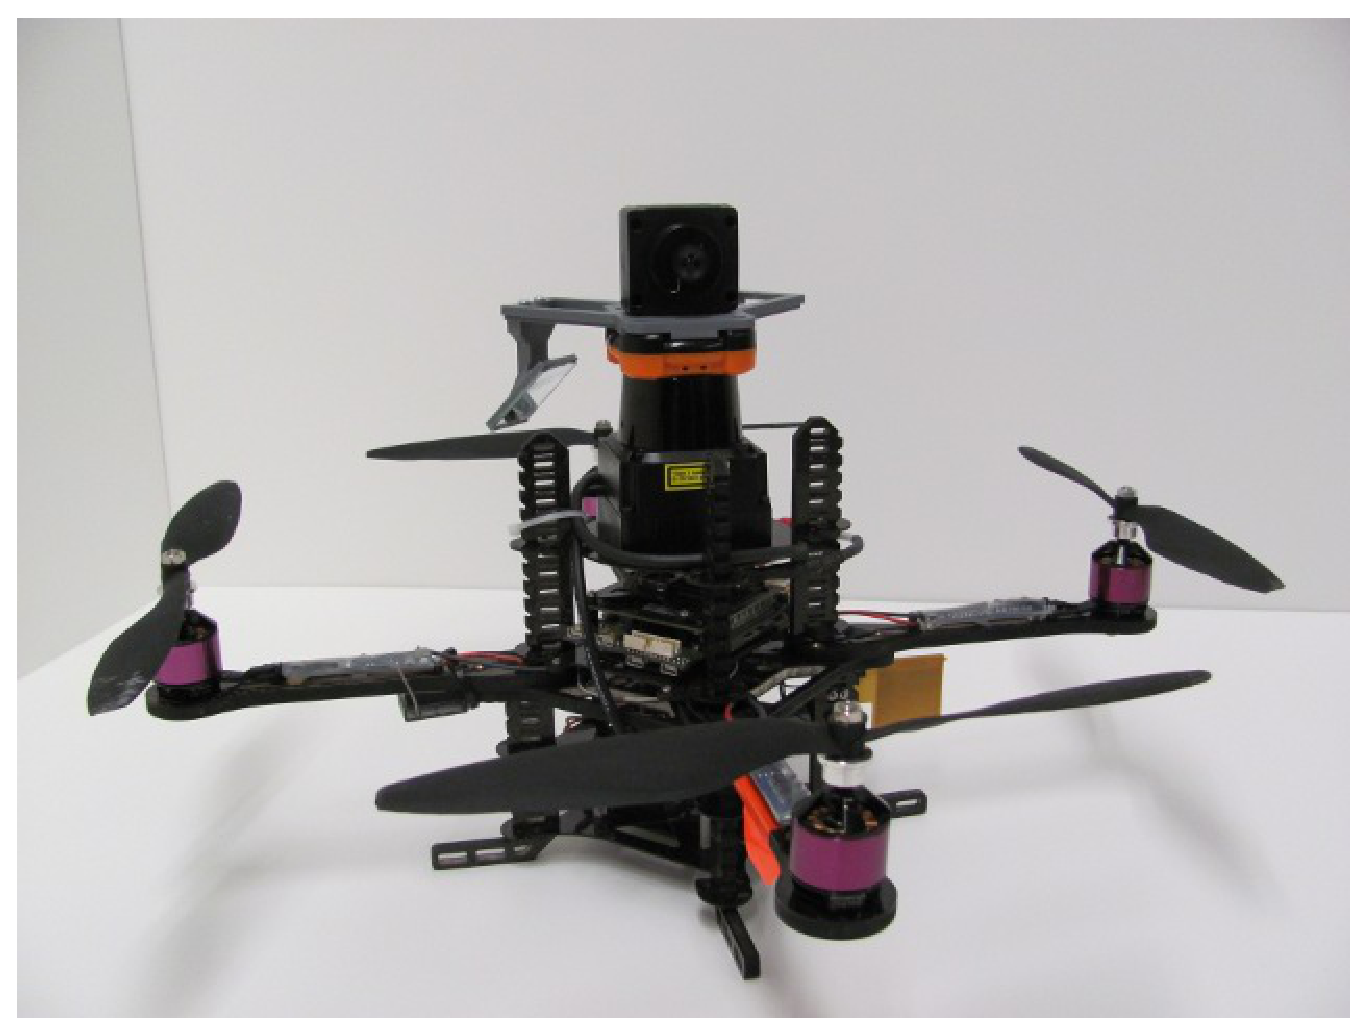
\includegraphics[width=0.5\textwidth]{images/pelican.eps}
	\caption{Ascending Technologies Pelican equipped with a camera and a laser scanner. The development is driven by commercial, government, research and military purposes. The small quadrotor allows remote observation of hazardous environments inaccesible for humans and ground robots.}
	\label{pelican}
\end{figure}

AR.Drone SLAM is a framework for the Parrot AR.Drone, a quadrotor, developed and proposed by N. Dijkshoorn. This framework contains a realtime Simultaneous Localization and Mapping (SLAM) implementation based on a down-pointing camera. Therefore, it allows a MAV to know its position and movement in the environment by generating a feature map of the environment so the MAV can localize itself on this map. Furthermore, the framework contains a 3D mouse controller, a keyboard controller, a visual map and an elevation map. Due to the framework the robot acquires more information of the environment. This information can aid the robot in navigation.

\subsection{Research questions and objectives}
In robotics one goal is to develop mobile robots that can advance robustly and truly autonomously in real world situations. One of the main requirements is the ability to navigate autonomously. Since there is no GPS signal available in urban and indoor environment, robots need to rely on other sensors.

Line-following is proven to be a simple navigation task for ground robots. However, this navigation task is not implemented yet on unmanned aerial vehicles. Since there are various linear structures in the environment, line-following should be a suitable navigation technique.

Therefore, the main research question is to find a robust vision-based approach to autonomously navigate over linear shaped structures. This main research question is divided up in the following sub-questions:
\begin{itemize}
\item What type of sensors should the AscTec Pelican carry?
    \begin{itemize}
        \item What type of down-pointing camera?
        \item What other sensors?
    \end{itemize}
\item How to port the framework AR.Drone SLAM to the AscTec Pelican?
\item How to detect and track a line?
\item What is the performance and robustness of different vision-based methods to navigation over a linear structure?
\item How should the vision-based algorithms be evaluated?
\end{itemize}
In order to perform line-following navigation, first, a line should be detected. Secondly, the angle between the quadrotor and the line is calculated. Finally, the quadrotor adjusts its movements in order to navigate over the line. These steps are repeated until the end of the line has been reached.
\subsection{Outline}
Chapter X gives an overview about currently used vision-based methods...
To be written.



\end{document}
